\documentclass{article}
\usepackage{amsmath}
\usepackage{graphicx} 

\title{Mathematics for Economics}
\author{Lajos Galambos}
\date{August 2024}

\begin{document}

\maketitle

\section{Introduction}
This is a note created for BA/MA level Mathematics for Economic Science based on the book of Knut Sydsæter and Peter Hammond: Essenatial Mathematics for Economic Analysis. This is part of my preparation for PhD application, and in general, to revise everything that is necessary to become an economist. 

\section{Algebra}
Natural Numbers – Integers – Rational Numbers – Irrational Numbers [infinite non periodic decimals] – Real Numbers

\subsection{Integer Powers}
\begin{equation}
  a^n = a \times a \times \ldots \times a \quad \text{(n times)}
\end{equation}

\begin{equation}
  a^0 = 1 \quad \text{for } a \neq 0
\end{equation}

\begin{equation}
  a^{-n} = \frac{1}{a^n}
\end{equation}

\subsection{Properties Powers}
\begin{equation}
  a^r \times a^s = a^{(r+s)}
\end{equation}

\begin{equation}
  (a^r)^s = a^{(r \times s)}
\end{equation}

\begin{equation}
  \frac{a^r}{a^s} = a^{(r - s)}
\end{equation}

\begin{equation}
  (ab)^r = a^r \times b^r
\end{equation}

\begin{equation}
  \left(\frac{a}{b}\right)^r = \frac{a^r}{b^r}
\end{equation}

\begin{equation}
  (abcde)^r = a^r \times b^r \times c^r \times d^r \times e^r
\end{equation}

\begin{equation}
  (a+b)^r \neq (a \times b)^r
\end{equation}

\subsection{Rules of Algebra}
In algebraic expressions, polynomials are defined by: \textbf{numerical coefficients}, and \textbf{terms of same type}. We can use \textbf{factoring} to make expressions more convenient to read. \\

Quadratic identities:
\begin{equation}
  (a+b)^2 = a^2 + 2ab + b^2
\end{equation}

\begin{equation}
  (a-b)^2 = a^2 - 2ab + b^2
\end{equation}

\begin{equation}
 (a+b)(a-b) = a^2 - b^2
\end{equation}

\subsection{Fractions}
Rules of fractions: 

\begin{equation}
 \frac{a\times c}{b\times c} = \frac{a}{b} \quad \text{for } b \neq 0 \text{ and } c \neq 0
\end{equation}

\begin{equation}
 \frac{-a}{-b} = \frac{a}{b} 
\end{equation}

\begin{equation}
 -\frac{a}{b} = \frac{-a}{b} 
\end{equation}

\begin{equation}
 \frac{a}{c} + \frac{b}{c} = \frac{a + b}{c} 
\end{equation}

\begin{equation}
 \frac{a}{b} + \frac{c}{d} = \frac{ad + cd}{bd} 
\end{equation} \\

LCD is a technique, finding the Least Common Denominator. It is used in especially the case of equation (18). \\

\begin{equation}
 a + \frac{b}{c} = \frac{ac + b}{c} 
\end{equation}

\begin{equation}
 a \times \frac{b}{c} = \frac{ab}{c} 
\end{equation}

\begin{equation}
 \frac{a}{b} \times \frac{c}{d} = \frac{ac}{bd} 
\end{equation}

\begin{equation}
 \frac{a}{b} \div \frac{c}{d} = \frac{a}{b} \times \frac{d}{c} 
\end{equation}

\subsection{Fractional Powers}
Powers can be written in a fractional form (if in the power we have rational numbers). Those are square roots. 

\begin{equation}
  a^{\frac{1}{2}} = \sqrt{a} \quad \text{valid if } a \geq 0
\end{equation}

\begin{equation}
 \sqrt{a} \times \sqrt{b} = \sqrt{ab}
\end{equation}

\begin{equation}
 \sqrt{\frac{a}{b}} = \frac{\sqrt{a}}{\sqrt{b}}
\end{equation}

\begin{equation}
 \sqrt{a} + \sqrt{b} \neq \sqrt{a} + \sqrt{b} \quad \text{(in general)}
\end{equation}

\begin{equation}
 a^{\frac{1}{n}} = \sqrt[n]{a} 
\end{equation}

\begin{equation}
 a^{\frac{p}{q}} = (\sqrt[q]{a})^p = \sqrt[q]{a}^p  \quad\text{(p an integer, q a natural number)}
\end{equation}

\subsection{Inequalities}

(1) If the two sides of an inequality are multiplied by a positive number, the direction of the inequality is preserved.
(2) If the two sides of an inequality are multiplied by a negative number, the direction of the inequality is reversed.

\begin{equation}
 \text{If } a > 0 \text{ and } b > 0, \text{ then } a + b > 0 \text{ and } a \times b > 0
\end{equation}

\begin{equation}
 \text{If } a > b, \text{ then } a - b > 0
\end{equation}

\begin{equation}
 \text{If } a \geq b, \text{ then } a - b \geq 0
\end{equation}

\begin{align}
 \text{If } a > b \text{ and } b > c, \text{ then } a > c \\
 \text{If } a > b \text{ and } c > 0, \text{ then } a \cdot c > b \cdot c \\
 \text{If } a > b \text{ and } c < 0, \text{ then } a \cdot c < b \cdot c \\
 \text{If } a > b \text{ and } c > d, \text{ then } a + c > b + d
\end{align} 

\begin{figure}[h]
\centering
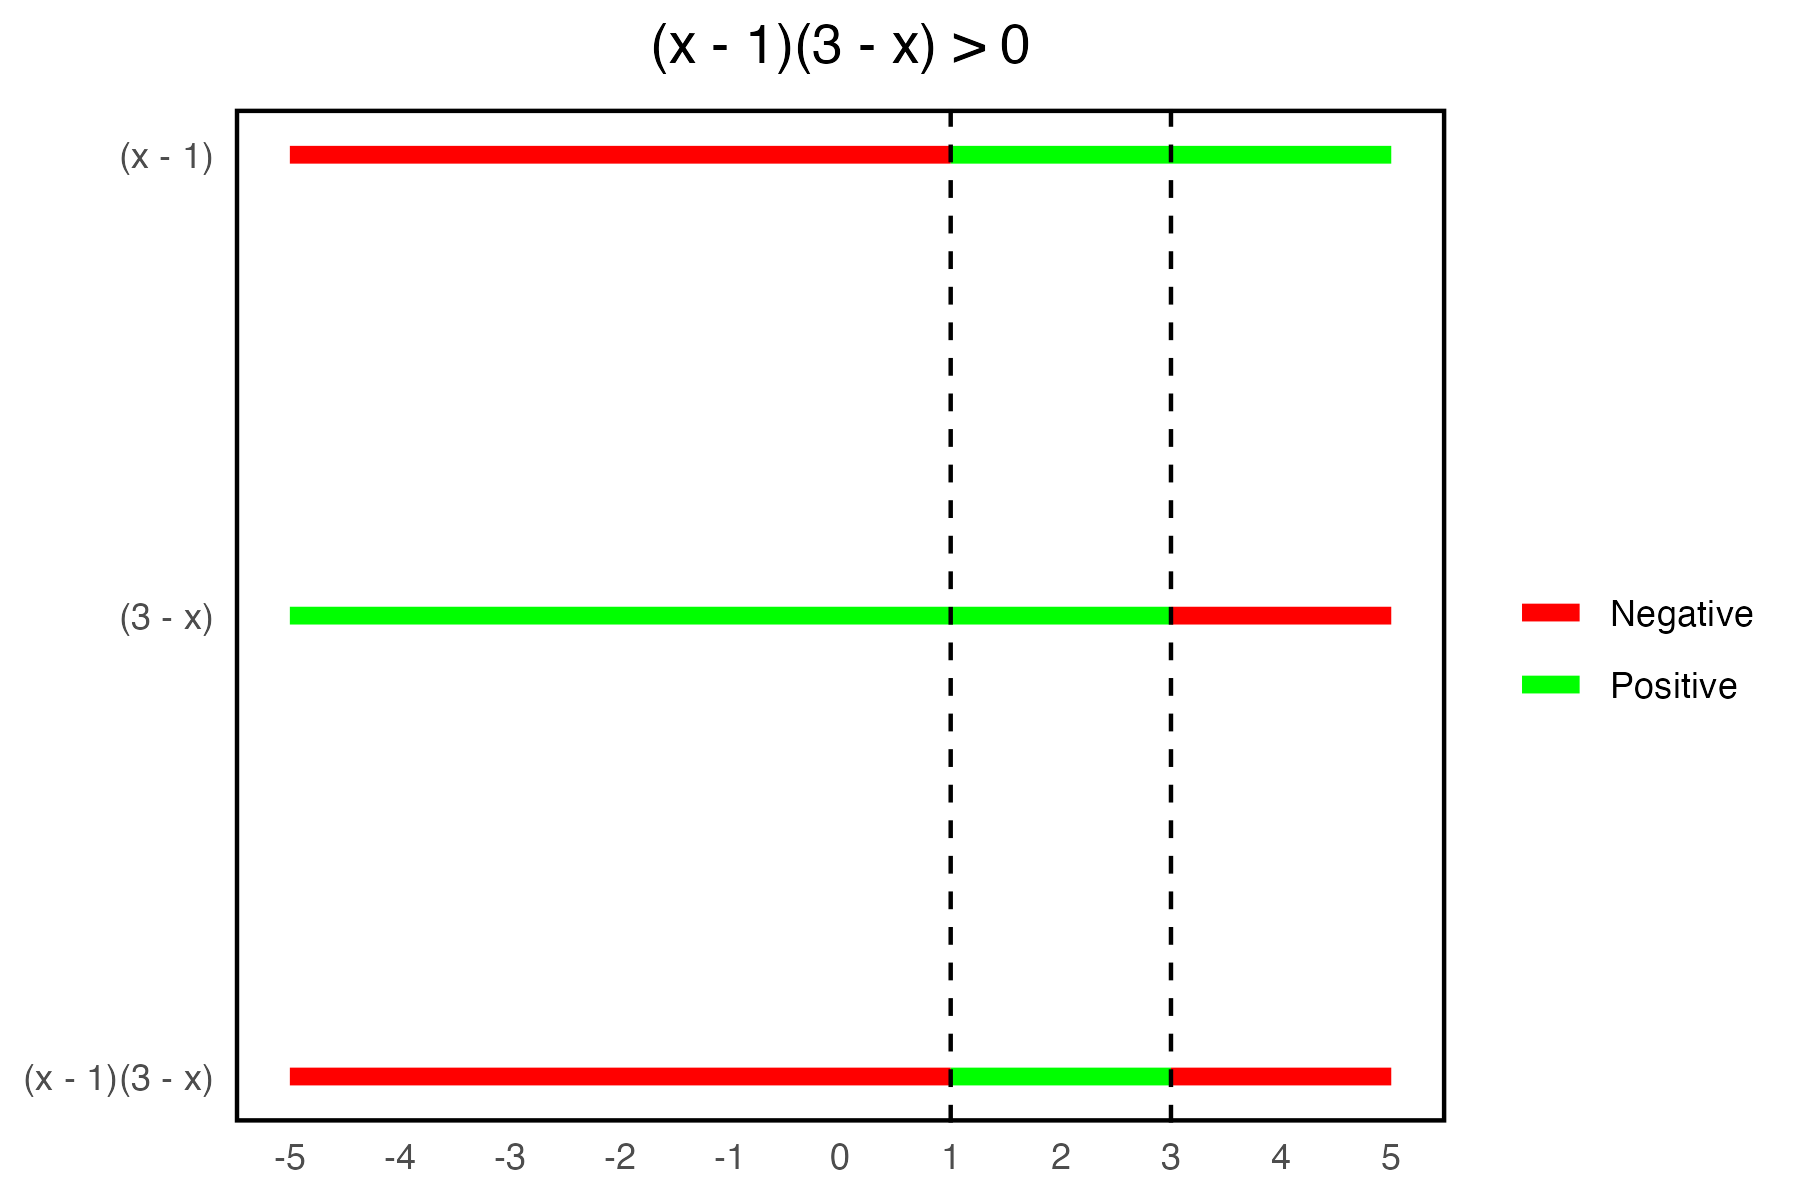
\includegraphics[width=0.8\textwidth]{Sign_Diagram.png}
\caption{Sign Diagram}
\end{figure}

Two inequalities that are valid simultaneously are often written as a \textbf{double inequality}. If, for example, \(a \leq z\) and moreover \(z < b\), it is natural to write \(a \leq z < b\). \\

\subsection{Intervals}
\begin{table}[h]
\centering
\caption{Notation of Intervals} 
\begin{tabular}{l|l|l}
\hline
Notation & Name & The interval consists of all x satisfying: \\
\hline
(a, b) & The open interval from a to b. & $a < x < b$ \\
\hline
[a, b] & The closed interval from a to b. & $a \leq x \leq b$ \\
\hline
(a, b] & A half-open interval from a to b. & $a < x \leq b$ \\
\hline
[a, b) & A half-open interval from a to b. & $a \leq x < b$ \\
\hline
\end{tabular}
\end{table}



\end{document}